\documentclass[conference]{IEEEtran}

\usepackage{ulem} 
\usepackage{subfigure}
\usepackage{comment}
\usepackage{graphicx}
\usepackage{algorithm}
\floatname{algorithm}{Procedure}
\usepackage{multirow}
\usepackage{makeidx}
\usepackage{amsmath}
\usepackage{amssymb}
\usepackage{epsf}
\usepackage{pstricks}
\usepackage{pst-grad}
\usepackage{placeins}
\usepackage{url}
\usepackage{epsfig}
\usepackage{multirow}
\usepackage{pifont}
\usepackage{graphics}
\usepackage{color}
\usepackage{epsf}
\usepackage{mathcomp}
\usepackage{colordvi}
\usepackage{epsfig}
\usepackage{fancyhdr}
\usepackage{wasysym}
\usepackage{longtable}
\usepackage{afterpage}
\usepackage{colordvi}
\usepackage{latexsym}
\usepackage{float}
\usepackage{alphalph}
\usepackage{epic,eepic}
\usepackage{authblk}
\usepackage{algpseudocode}
\usepackage{mathptmx}
\usepackage{epstopdf}
\usepackage[justification=centering,font=normalsize,labelfont=bf]{caption}
%\captionsetup{aboveskip=4pt}
%\usepackage{flushend}

\algnewcommand{\LineComment}[1]{\State \(\triangleright\) #1}

\renewcommand{\baselinestretch}{1.01}

\newtheorem{definition}{Definition}
\newtheorem{example}{Example}
\newtheorem{note}{Note}
\newtheorem{operation}{Operation}
\newtheorem{axion}{Axion}
\newtheorem{remark}{Remark}
\newtheorem{lemma}{Lemma}
\newtheorem{theorem}{Theorem}

\ifCLASSINFOpdf
  % \usepackage[pdftex]{graphicx}
  % declare the path(s) where your graphic files are
  % \graphicspath{{../pdf/}{../jpeg/}}
  % and their extensions so you won't have to specify these with
  % every instance of \includegraphics
  % \DeclareGraphicsExtensions{.pdf,.jpeg,.png}
\else
  % or other class option (dvipsone, dvipdf, if not using dvips). graphicx
  % will default to the driver specified in the system graphics.cfg if no
  % driver is specified.
  % \usepackage[dvips]{graphicx}
  % declare the path(s) where your graphic files are
  % \graphicspath{{../eps/}}
  % and their extensions so you won't have to specify these with
  % every instance of \includegraphics
  % \DeclareGraphicsExtensions{.eps}
\fi

\hyphenation{op-tical net-works semi-conduc-tor}
\begin{document}

\title{Reducing Display Power Consumption for Real-time Video Calls on Mobile Devices}

%%
%% Reducing Display Power Consumption for Real-time Video Calls on Mobile Devices
%% Design and Implementatin of a Practical/Greedy Power Saving Scheme for Real-time Video Calls on Mobile Devices
%% =================
%% Adaptive Display Scheme over Real-time Multimedia Communication on Mobile Devices
%%

%for single author (just remove % characters)
%%\date{}
%% \special{papersize=8.5in,11in}
%% \setlength{\pdfpageheight}{\paperheight}
%% \setlength{\pdfpagewidth}{\paperwidth}

%% \conferenceinfo{Submission to SoCC '14}{October, 2014, Seattle, WA, USA} 
%% \copyrightyear{2014} 
%% \copyrightdata{978-1-nnnn-nnnn-n/yy/mm} 
%% \doi{nnnnnnn.nnnnnnn}


%% \author{
%%   \IEEEauthorblockN{Mengbai Xiao}
%%   \IEEEauthorblockA{
%%     mxiao3@gmu.edu\\
%%     Department of Computer Science\\
%%     George Mason University}
%%     \and
%%   \IEEEauthorblockN{Songqing Chen}
%%   \IEEEauthorblockA{
%%     sqchen@gmu.edu\\ check the email\\
%%     Department of Computer Science\\
%%     George Mason University}
%% }

\author{}

\maketitle

%\thispagestyle{empty}

%\sloppy
%------------------------------------------------------------------------------

\begin{abstract}

On a mobile device, the display subsystem ususally consumes 30\%-60\%
of the total battery power.  As such, a few designs have aimed to
reduce the display power consumption in mobile video streaming.  The
basic idea is to dim the backlight level while properly compensating
the pixel luminance to maintain image fidelity.  The luminance
compensation and proper luminance calculation are computation
intensive and demand per-frame luminance information. Thus, existing
schemes only target video-on-demand where the luminance information of
each frame is available in advance. In addition, they demand
additional computing resource support. Otherwise, if the computation
is conducted on the mobile device, the computing
overhead can easily offset the power saving.  In this work, we set to
investigate power saving for video calls on mobile devices.  Different
from video-on-demand, the real-time video calls are highly delay
sensitive and the frame luminance information is not known in
advance. Moreover, video calls often involve multiple
streaming sources from multiple ($\ge$2) participants, making it more
difficult.  Because there are fewer background changes and a often
slower frame rate in video calls, we design a greedy display power
saving scheme, called LCD-GDP, by utilizing the commonly available GPU on mobile
devices without demanding additional support.  Our design is
implemented on WebRTC, a popular real-time web browser based video
call standard.  Experiments show that our scheme can save upto 40\%
power consumption in video calls.

%% Power saving is a significant issue at the mobile platform. Various
%% techniques were proposed to extend the playback time of the
%% videos. Backlight scaling is one of them and target the display
%% subsystem. However, the multimedia content need to be delivered in a
%% timely manner in the real-time communication. This raises challenges
%% towards the existing backlight scaling technique. The backlight
%% scaling technique is composed of computation intensive tasks,
%% including the luminance histogram generation and the pixels
%% luminance compensation on every frame. Multiple streaming sources in
%% the video conference make this problem more difficult. Moreover,
%% global luminance information is necessary for finding the optimal
%% backlight levels across the streaming. This is clearly impossible in
%% the real-time case. In this paper, we propose a greedy algorithm
%% determining the backlight level of current frame only from the last
%% one. We also take advantage of the GPU to relive the burden of the
%% CPU on compensating the luminance of pixels. We integrate our
%% prototype in the AppRTC, an Android app based on WebRTC, and find
%% that our scheme can save up to 39.8\% energy during one
%% communication session.
\end{abstract}


%\vspace{-1em}
\section{Introduction}


With the ever-improving network and mobility support, recently,
real-time communication software, being standalone or combined with
social media, have also found their way on mobile devices.  Being able
to support video calls while entirely free or at least cheaper than
the traditional voice communications, these software, such as
Skype~\cite{skype}, QQ~\cite{qq}, Apple's Facetime~\cite{facetime},
and Google WebRTC~\cite{webrtcproject}, are quickly gaining popularity
among common mobile users.


However, the limited battery power supply remains as the Archille's
heels of mobile devices while real-time video communications are very
power-hungry. Compared to the video streaming, real-time video calls
are more demanding. In the real-time video communication, such as the
video conferencing, the video contents are generated on the fly from
multiple sources. Even for the one-to-one video call, double frames
are generated other than the common video streaming. Thus, efficiently
reducing the power consumption for video calls on mobile devices is
imperative.


Previously, since the display subsystem on a mobile device often
consumes about 38\% to 68\% of the total energy during video
streaming~\cite{AG10}, a few schemes have been designed to reduce the
power consumption of the display. For a Liquid-Crystal Displays (LCD)
display, the dominant power consumption is by the backlight
intensity. Thus to reduce the power consumption, it is desirable to
dim the backlight as much as possible while enhancing the luminance of
the pixels to comprensate the quality degradation due to backlight
dimming.  In this way, the modified images on the screen can maintain
image fidelity to the human's eyes. Such a technique is called
backlight scaling.

In detail, the backlight scaling technique often consists of three
stages, i.e., 1) the histogram generation stage, 2) the backlight
levels determination stage, 3) the pixel compensation stage. The first
stage and the last stage are both computation intensive. Therefore,
some previous design either ignore the luminance
compensation~\cite{HLH11}, leading to significant quality degradation
and user experience unsatisfaction, or demand additional computing
resources for compensation~\cite{LHH14}, making the scheme
non-practical for mobile devices.  In the second stage, some previous
research applies the dynamic programming to find the globally optimal
backlight levels without violating the hardware and user experience
constraints. Thus, the video frames must be available in advance.
However, for real-time video calls, this is impossible because the
video content is generated on the fly.  Furthermore, being higly
sensitive to delay, real-time video calls cannot tolerate the delay
that may be caused by the dynamic programming. In addition, by often
supporting multiple participants and thus receiving data from multiple
sources simultaneously, the backlight scaling technique cannot be
directly used for video calls.

In this paper, we set to explore the display power saving for video
calls on mobile devices. Since there are often less background changes
and slower frame rate in practical video calls, we propose a greedy
display power saving scheme, called {\it LCD-GDP}.  Similar to the dynamic programming
approach for video streaming, there are same constraints that our
greedy algorithm must conform to. The {\it first} is that the backlight
variations between neighboring frames must be limited. Otherwise the flickering effect is expected
in the user experience~\cite{}. {\bf add reference here} The {\it second} is that the backlight should not be
scaled down too much to cause image distortion~\cite{}. {\bf add
  reference}  The {\em third} is that the
backlight cannot be adjusted too frequently because the hardware needs some time
to respond~\cite{}. {\bf add reference}


To avoid processing the same frame repeatedly, in LCD-GDP, {\it first}, we migrate
the histogram generation to the sender side for video calls. We
put the luminance information inside each frame without building an
additional channel. Also duplicated information is hidden for the
possible loss during the video encoding/decoding and the network
transmission.

{\it Second}, since GPU is commonly equipped in the mobile devices, we
take advantage of GPU to offload some tasks from the
CPU. For the purpose of rendering the received frames in a timely
manner, we use the OpenGL ES 2.0 shaders to perform the pixel
enhancement.  Moreover, the power savings will not be offset by
enabling GPU since GPU is widely used in the video conferencing for
composing frames together and then rendering them.

To evaluate the performance of our design, we implement LCD-GDP into
WebRTC and run experiments on a tablet and a smartphone. Experimental
results show that {\bf by using the LCD-GDP, the metric of frames per
  second doesn't decrease obviously and only additional tens of
  milliseconds are found in latency. Upto $33.2\%$ power consumption
  can be saved on average due to the brightness of the
  environment. }

This paper is organized as follows. We describe some background
information for both backlight scaling and WebRTC 
%is introduced and some related work is reviewed 
in Section \ref{sec:background}. We present
our design in Section \ref{sec:design} and the implementation details
in Section \ref{sec:implementation}. We discuss
the evaluation in Section \ref{sec:evaluation} and conclude our work
in Section \ref{sec:conclusion}.


%% old representation
\if 0
The great success of the real-time communication has been witnessed in
the last decade. The popular software, like Skype, QQ and Apple's
Facetime, make the real-time communication as a cheaper alternative to
the calls. Nowadays, with the emerging mobile market, these
applications were migrated to the mobile platform as well. However,
like the other mobile applications, the power issue is hindering the
deployment of real-time communication on the mobile
devices. Especially in the real-time communication app, several
power-hungry modules, like wireless network, camera and etc. So
maximizing the power savings is desired and attractive in the
real-time communication.


According to the previous research ~\cite{AG10}, about 38\% to 68\% of the
total energy is consumed by the display subsystem during the video
playback, and this portion is growing on the new generation of
devices, which are equipped with more powerful GPUs and more
large-sized display panels. We also expected the average power
consumption during the real-time communication will be cut down if the
display subsystem is optimized. One existing technique, named
backlight scaling, can be used to reduce the energy consumption of
Liquid-Crystal Displays (LCD). The power consumption of LCD is
dominated by the backlight intensity, so this technique tries to dim
the backlight as much as possible while enhancing the luminance of the
pixels, which are rendered on the screen, at the same time. In this
way, the modified images on the screen are perceived as the original
ones by the human eye.  


In this paper, we explored the possibility of deploying the backlight
scaling technique with the real-time communication. The backlight
scaling technique is composed of three stages. 1) Histogram generation
stage. 2) Backlight levels determination stage. 3) Pixels compensation
stage. The first stage and the last stage are both computation
intensive tasks when performing these operations on each frame. In the
second stage, previous research applies the dynamic programming to
find the globally optimal backlight levels without violating some
constraints. Not only is the extra CPU time required, but also the
backlight levels can be determined on-the-fly. All of these obstruct
the backlight scaling technique being applied in the real-time
communication.

In the real-time communication, like the video conferencing, the video
contents are generated from multiple sources. Even for the one-to-one
video call, double frames are generated other than the common Internet
streaming, like watching the movies. To avoid processing the same
frame repeatedly, we migrate the histogram generation stage to the
sender side. We put the luminance information inside each frame
without building an additional channel. Also duplicated information is
hidden for the possible loss during the video encoding/decoding and
the network transmission.

The dynamic programming algorithm is necessary in the common video
playback scenario since there are some constraints we have to conform
to. The backlight variations must be limited when the flickering
effect is not expected in the user experience. Also the backlight
should not be scaled down too much to cause the distortion. However,
the dynamic programming is not applicable in real-time communication
due to the dynamically generating video contents. Even if this
algorithm is partially applied, significant delays are introduced in
the sessions. Fortunately, in the real-time communication, we can risk
scaling the backlight levels in greedy manner because no scenes
switching are expected. 

When the GPU is commonly equipped in the mobile devices, we are able
to take advantage of this facility to offload some tasks from the
CPU. For the purpose of rendering the received frames in timely
manner, we use the OpenGL ES 2.0 shaders to perform the pixels
enhancement stage. Little delays are introduced in this way. Moreover,
the power savings won't be offset by enabling GPU since GPU is widely
used in the video conferencing for composing frames together and then
rendering them.

This paper is organized as follows: the background is introduced and
some related work is reviewed in Section \ref{sec:background}. We propose
our design in Section \ref{sec:design}. The details of implementation
are illustrated in Section \ref{sec:implementation}. Then we discuss
the evaluation in Section \ref{sec:evaluation} and conclude our work
in Section \ref{sec:conclusion}.
\fi


%% The real-time communication, as a considerably
%% cheaper alternative to the calls, makes QQ, Skype, Apple's
%% Facetime and etc. so popular all round the world. More attractively,
%% with the bandwidth growth of the Internet, the real-time communication
%% is always equipped with the video channel so that two ends can talk
%% face-to-face. Now the prosperity of mobile devices, including
%% smartphones, tablets and emerging wearable devices, offers another
%% available platform for the real-time communication. The real-time
%% communication is more desired on these portable devices, which can
%% benefit from the wireless networks everywhere. However, new challenges
%% to deliver video stream on the mobile devices have raised and one of
%% them is to maximize the power savings.


% stress the importance real-time communication on mobile devices
% This part is redundant, make it concise.
% Don't discuss the details of WebRTC. Only mention the general idea
% of Real-time communication.


%% On the other hand, Dynamic Adaptive Streaming over
%% HTTP(DASH) makes a salient example that how multimedia streaming is
%% delivered nowadays. WebRTC(Web Real-Time Communication), technique
%% that integrating real-time communication over HTTP, is standardized by
%% W3C and the IETF. Thus a cross-platform solution will be handy and the
%% growth of real-time communication on new platform is
%% expected.
%% As an advanced functionality, video call becomes an essential
%% component in many *communication applications/wechat, skype... check
%% in twin cloud paper*. The needs for unifying the interface is
%% increasingly desirable. The success of DATH *add name* hints people
%% the importance of HTTP in video/audio streaming scenarios. WebRTC as a
%% new API existing in HTML5 drops in developer's sight. Mainstream
%% browsers integrates the function into there production, i.e. Chrome,
%% Opera, Firefox. Developers can easily include video call in their page
%% via few lines of javascript code.


%% In this paper, we explored the possibility if an effective LCD
%% power-saving technique, named luminance compensation, can be applied
%% on the real-time communication services. There are three steps in this
%% technique. 1) Extract the luminance histrogram of the frames. 2)
%% Decide the backlight levels and do scaling when the frames are
%% rendered. 3) According to the backlight levels, enhance the luminance
%% component of the pixels. This technique has been successfully adopted
%% on some other streaming services, however, there are still 
%% several challenges in the real-time case:
%% \begin{itemize}
%%   \item
%%     {
%%       Unlike the other streaming services of predefined content, in
%%       real-time communication, there is no way to build a utility to
%%       extract and analyze the videos in the offline manner. The extraction
%%       process, which is computation intensive, has to be installed
%%       along with the services. 
%%     }
%%   \item
%%     {
%%       In a N-party communication, $N$ frames are rendered on one screen
%%       at the same time. $N$ times the input data makes the extraction
%%       operation even worse.
%%     }
%%   \item
%%     {
%%       To decide the backlights levels, a dynamic programming algorithm
%%       has been proposed. However, this handy soloution requires large
%%       buffer size to collect enough luminance information and then to
%%       reach the global optimal result. However, this is not practical
%%       in the real-time case.
%%     }
%% \end{itemize}

%% designed a system composed three components in the names of {\bf
%%   Scanning Module}, {\bf Adjustment Module} and {\bf Rendering
%%   Module}. These components are integrated into real-time
%% communication.


% conventional
%% On the other hand, people doesn't satisfy themselves with traditional
%% phone call, which make them only listen to their relatives. On
%% smartphone, installing communication applications becomes available
%% and people can also see the other end over one call. *not only on the
%% traditional PC*. Moreover, video call is much cheaper, sometimes even
%% free. In the future day, we can easily make video call over webRTC,
%% the unifying interface in browsers. Since both on the mobile and PC we
%% can access it via browsers. Even more, Google has been making effort
%% on packaging their implementation in Chrome as available for Android
%% App developers. So we can make such call via the simple thing.

%% The power-saving scheme for VoIP is few, since the most applications
%% are properties of company. Researchers is hard to figure out which
%% part is enable to save the energy. Also the old applications are
%% designed for PC client. The achievement is in the network layer,
%% adapting the transmission protocols to specific scenarios *I guess,
%% check it*. On the other hand, many effective energy effective schemes
%% were proposed for streaming on mobile platform, such as *give some
%% example, ref to our paper*. This motivate us to put these schemes in
%% the real-time multimedia case.

%% Thanks to Google, the Chromes is an open source project, in the nature
%% of things the WebRTC is part of it as libjingle*introduce to
%% libjingle*. More fortunately, the libjingle is able to be integrated
%% as 3rd library with Android applications. So the Android application
%% can take advantage of this aside web browsers.

%% Display is the most great part of mobile power consuming. As
%% LCD*introduce the LCD?*, one 
%% efficient way to save power is adjust the backlight with compensating
%% the pixels. there are works done on the local video case and online
%% streaming case. Usually the GPU is used to dynamically scan frames and
%% retrieve the highest pixels. we have some opportunities:
%% \begin{itemize}
%%   \item
%%     {
%%       % Challenge: Cooperation
%%       In the real-time case, or the p2p case, video is generated via
%%       clients. We don't need to passively accept the frame and parse
%%       frames until them are decoded. On the other hand, we can scan
%%       the frames before encoding when the stream is
%%       generated. How can we effectively do this? one challenge is how
%%       we pass the information to the other side. we
%%       don't need to open another data channel on this. put the max
%%       pixel at the corner.
%%       *We can also split the scanning process*
%%       we offload the DP part to the receiver.
%%     }
%%   \item
%%     {
%%       % Challenge: take advantage of the scenarios
%%       Also the real-time communication has its characteristics. The
%%       frames staying relative still. We can adjust the max liminance
%%       in greedy manner. More aggressively, we can adjust the frames
%%       in case of skipping some frames. 
%%     }
%%   \item
%%     {
%%       % Challenge: graphical composition
%%       The receiver is asked to compose frames received from several
%%       senders. 
%%     }
%%   \item
%%     {
%%       % The DP problem
%%       The DP is not optimal if the power-backlight is not linear
%%       relationship. But the Greedy is even more not optimal.

%%       In real-communication users is more likely to be tolerant. 
%%     }
%% \end{itemize}




%\vspace{-1em}

\section{Background}
\label{sec:background}
In this section, we briefly introduce the backlight scaling and WebRTC
for real-time video calls.

\subsection{Backlight scaling}
A visible image on a LCD display is produced by both backlight and the LCD
panel, which stores pixel color imformation. The perceptual luminance
is actually the backlight intensity compensated by the pixels. The
backlight scaling is a technique  exploiting
this characteristic. 
{\bf do we have another figure? captured from playing other videos? If
we do, can replace. But can delay till the last minute.}
Figure~\ref{fig:backlightscaling} sketches the high-level idea. As
shown in the figure, the energy for displaying the image can be
reduced by dimming the backlight. If  nothing else is done, 
 it will lead
to a darker version of this image. This distortion can be compensated
by concurrently increasing the luminance component of each pixel in
this image~\cite{PMLDV03, CHP07, CCS06, CSC02}. And increasing the
pixel brightness does not increase the power consumption of the
display.


\begin{figure}[!htb]
  \begin{center}
    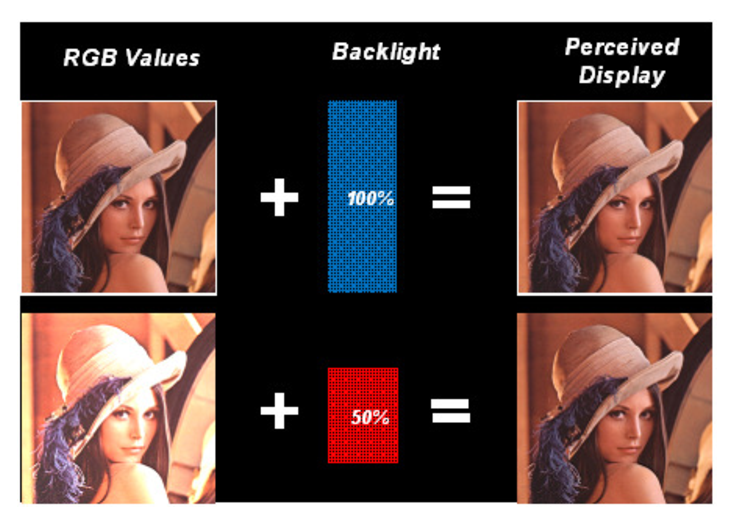
\includegraphics[scale=.75]{./figures/backlightscaling.eps}
    \caption{Backlight Scaling on LCD screen}
    \label{fig:backlightscaling}
  \end{center}
\end{figure}

However, directly applying backlight scaling to video playback faces
several challenges. Both extracting and enhancing the pixels luminance
component frame by frame demand processing a mass of data, and is
computation intensive.  For this reason, deploying these tasks during
the playback on the same CPU~\cite{CHP07, CSC02} is not practical
because of two reasons.  On the one hand, the CPU may not have enough
time to perform these computation intensive tasks without degrading
the video quality (e.g., frames per second or FPS) of the video playback. On
the other hand, the achieved power saving by dimming the backlight can be
offset by the power consumption due to these extra CPU operations. Hsiu et al. and Lin et
al.~\cite{LHH14, HLH11} proposed to skip the pixel compensation stage
and use a critical backlight level for each frame to avoid distorting
the image too badly. Ruggiero et al. suggested to offload the
luminance adjustment tasks to the hardware image processing unit (IPU)
integrated in Freescale’s multimedia application
processor~\cite{RBB08}. It exploits in a smart and efficient way to
implement a hardware assisted image compensation.
%% {\bf is this processor on the same machine or
%%   different machine?} 
Pasricha et al.~\cite{PMLDV03} and Cheng et al.~\cite{CMEDV07}
suggested to compute the backlight scaling data on a proxy server and
substitute the original video with a luminance-adjusted version. In
short, existing schemes (1) only target video-on-demand where the
video frame information is available in advance so that the computing
can be done before the playback, and (2) demand additional
infrastructure support for compensation or do not consider quality
degradation due to backlight dimming. So far, no scheme has been
considered for real-time video calls.

Compared to video-on-demand, real-time video calls are live streaming,
where each frame is produced on the fly and highly
delay-sensitive. Furthermore, video calls often invovle
multiple participants, and thus multiple frames from different sources
needed to be combined in real-time, leaving little computing power for
other tasks, such as pixel luminance compensation.

\subsection{Video Calls and WebRTC}

Video calls/conferecing are gaining increasing popularity.  On mobile
devices, many applications, such as Skype, QQ, and
Facetime~\cite{skype, qq, facetime}, {\bf this is not proper. add
  reference to each separately} all support video
calls/conferecing. The communication protocol of these applications is
proprietary to commercial companies, which precludes the communication
between different applications.  The increasing varities of mobile
devices, such as smartphones, tablets and emerging wearable devices,
make the situation even more complicated. To solve this fragmentation
problem in the real-time multimedia communication and also to provide
a cross-platform solution, Web Real-Time Communication
(WebRTC)~\cite{webrtcstandard} is proposed to enable video
communications via web browsers and standardized by the W3C and
IETF. Nowadays, mainstream browsers, e.g., Chrome, Firefox, Opera, all have integrated the WebRTC. The WebRTC
component~\cite{webrtcproject} implemented in the Chrome provides the
Javascript-style APIs. WebRTC can be linked to the native mobile apps
as an external libary.  WebRTC is now widely used by mobile
users. {\bf do you have some data about usage to put here? with
  references.} {\bf revise this later} However, given its video
streaming nature, the power consumption of video communication is
high, which has slowed down its pervasion.



%%% old 
%% \section{background}
%% \label{sec:background}

%% \subsection{Backlight scaling}
%% A visible image on LCD display is produced by both backlight and LCD
%% panel, which stores pixels color imformation. The perceptual luminance
%% is actually the backlight intensity compensated by the pixels. The
%% backlight scaling is a dedicated technique for LCD screen exploiting
%% this characteristics. This technique can be clearly illustrated in the
%% figure~\ref{fig:backlightscaling}. The energy of displaying one
%% picture can only be reduced by dimming the backlight, though it leads
%% to a darker version of this image. This distortion can be compensated
%% by concurrently increasing the luminance component of each pixel in
%% this image~\cite{PMLDV03, CHP07, CCS06, CSC02}. Fortunately, the
%% pixels brightness is uncorrelated to the power consumption of the
%% display.


%% \begin{figure}[!htb]
%%   \begin{center}
%%     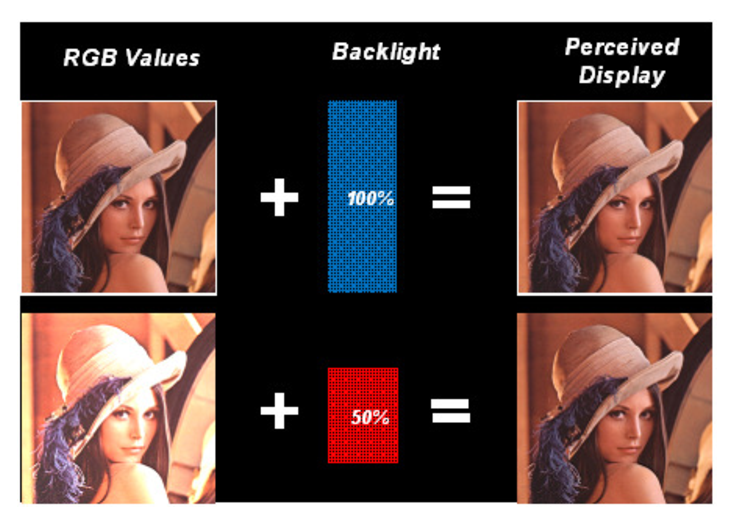
\includegraphics[scale=.75]{./figures/backlightscaling.eps}
%%     \caption{Backlight Scaling on LCD screen}
%%     \label{fig:backlightscaling}
%%   \end{center}
%% \end{figure}

%% Applying this technique in the video playbacks raises several
%% challenges. Both extracting and enhancing the pixels luminance
%% component frame by frame are the operations of processing a mass of
%% data. For this reason, deploying these tasks on the CPU~\cite{CHP07,
%%   CSC02} is not practical. On the one hand, the CPU may don't have
%% enough time to do these computation intensive tasks without degrading
%% the frames per second (FPS) of the video. On the other hand, the
%% achieved power savings by dimming backlight might be offset by these
%% extra operations. Hsiu et al. and Lin et al. ~\cite{LHH14, HLH11} proposed to
%% skip the pixels compensation stage and use a critical backlight level
%% of each frame to avoid distorting the image too badly. Ruggiero et
%% al. offload the luminance adjustment tasks to an independent
%% processor~\cite{RBB08}. Pasricha et al.~\cite{PMLDV03} and Cheng et
%% al.~\cite{CMEDV07} suggested to compute the backlight scaling data on
%% a proxy server and substitute the original video with a
%% luminance-adjusted version.


%% \subsection{WebRTC}

%% The conversational RTC protocols are the company proprietaries,
%% precluding the communication between different services.  The
%% prosperity of mobile devices, including smartphones, tablet
%% and emerging wearable devices, makes the situation more
%% complicated. To solve the fragmentation problem in the real-time
%% multimedia communication and also to provide a cross-platform
%% solution, Web Real-Time Communication (WebRTC)~\cite{webrtcstandard}
%% is proposed and standardized by the W3C and IETF. Nowadays, mainstream
%% browsers, e.g. Chrome, Firefox, Opera and etc., all have integrated
%% the WebRTC inside them. Not only does the WebRTC
%% component~\cite{webrtcproject} implemented in the Chrome provide the
%% Javascript-style APIs, but also it can be linked to the native mobile
%% apps as an external libary. In this paper, we build our prototype
%% based on the AppRTC, which is the Android version app incorperating
%% the WebRTC library.


\section{System Design}
\label{sec:design}
%In this section, we present our design of LCD-GDP.

\subsection{System Components}
As we discussed before, the backlight scaling generally involves three
steps for 1) generating the luminance histogram, 2) determining the
proper backlight levels and 3) compensating the pixel luminance. In
our system, we decouple them into the following three independent
modules: the {\bf Scanning} module, the {\bf Adjustment} module, and
the {\bf Rendering} module. Next we present our new approaches in
these three modules, respectively. Figure~\ref{fig:design} illustrates
the organization and interaction of these three modules.

\begin{figure}[t]
  \centering
%  \label{fig:design}
  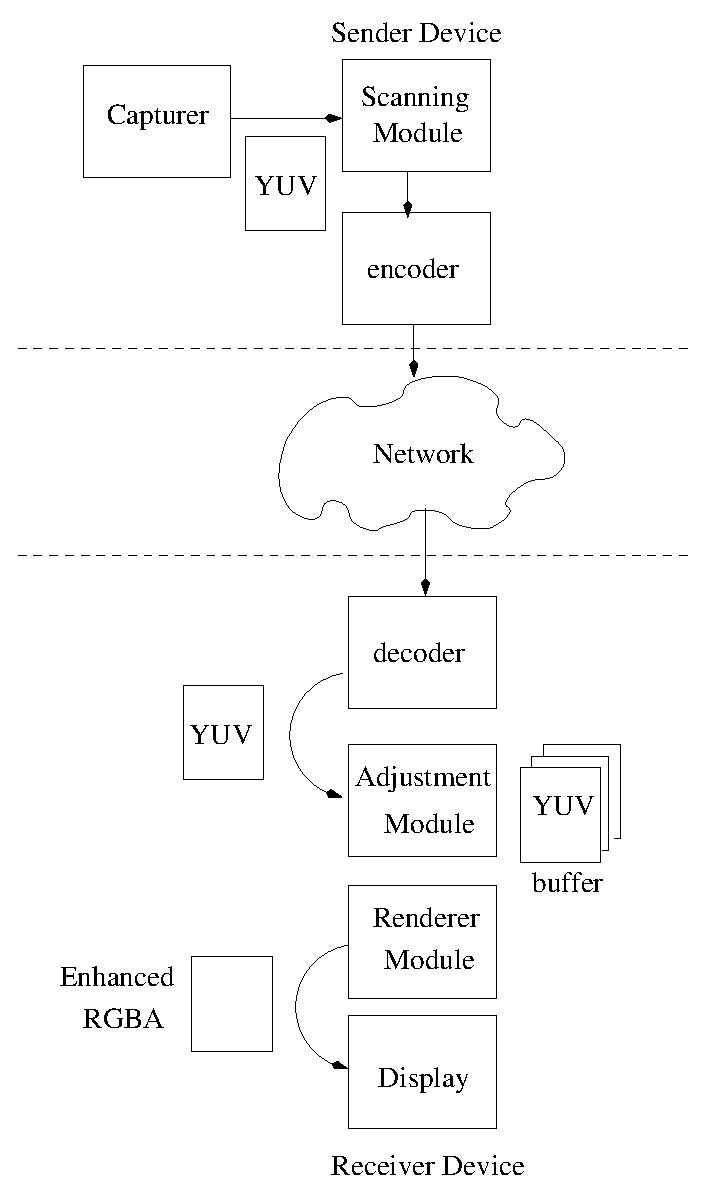
\includegraphics[width=.45\textwidth]{./figures/design.eps}
  \caption{LCD-GDP system architecture and major components}
\label{fig:design}
\vspace{-2em}
\end{figure}



\noindent{\bf Sender-Side Scanning and Piggybacking}:
The {\bf Scanning} module is the component to extract the pixel
luminance information. In the real-time communication, the frames are
generated by the capturer, which is usually a physical camera. There
is no way to access the whole video content in advance. So the
scanning module is necessary to generate the luminance histogram for
later determination stage and compensation stage. Other than the Video
On Demand (VOD), the RTC session involves $N \ge 2$ participants, and
the rendered image is composed by all received frames (including that
from the receiver itself). While it is natural to conduct the scanning
after receiving the image, in our design,  the scanning module is
installed at the sender side so that each generated frame will be
scanned only once. (Otherwise, every receiver needs to conduct the
scanning for the same image repetitively.)  However, this brings
another problem: how to transmit this luminance information to the
receivers if the scanning is done on the sender side. Building another
channel is possible, but it introduces additional overhead and extra
efforts must be made to synchronize the frames and the luminance
information. Either of them may not arrive the receiver on time.

To this end, we choose to encode this information with the frame data
for more efficiency on the luminance information transmission.  In our
scheme, the bottom corners are the best candidates. This position
either is covered by other frames, or is negligible when the frame is
resized to a smaller size.  Since the luminance information may also get
lost in the encoding process and network transmission, we propose to
duplicate this information and set them at the positions known by both
ends. The receiver side extracts the information and uses the maximum value
among the candidates, and then passes the value to the {\bf
  Adjustment} module for backlight scaling.

\noindent{\bf Greedy Luminance Adjustment}: The {\bf Adjustment} module is located at the receiver side. This
module aims to find the appropriate backlight levels from the
luminance information. In the VOD, global luminance information is
required to prevent the flickering effects, which is caused by scaling
the backlight with great variation too frequently--VOD usually
involves numerous scene switches. But 
 the real-time video communication is highly delay-sensitive, so buffering a certain
amount of frames for the purpose of waiting for enough luminance
information accumulated (and thus calculate the optimal backlight levels) is not
practical. In our design, we propose to use a greedy algorithm in the
determination stage, as we discuss in the next subsection. This
algorithm determines the current backlight level
only based on the latest information from the last frame. In this way,
little latency is likely to be introduced into the system. After this,
the new backlight levels are sent to the {\bf Rendering} module for
pixel compensation and backlight scaling.

\noindent{\bf GPU-assisted Rendering}:
The {\bf Rendering} module strengthens the original rendering function by
adding pixel compensation and backlight scaling.  In our design,
instead of using CPU, we choose the commonly available GPU on today's
mobile devices to enhance the pixel luminance.  For video calls,
typically the GPUs are enabled for resizing, composing the received
frames and performing RGB-YUV conversion. Thus,  little power consumption
cost is expected by the adding the pixel compensation task. This
module also scales the backlight levels to make the images on the
screen perceived by the user with no distortion from the original
version.

\subsection{Backlight Determination Algorithms}
Having discussed the system component, now we discuss the backlight
determination algorithm used for the {\bf Adjustment module}.

In general, before the $t$'th frame is rendered on the screen, the corresponding
backlight level $b_t$ must be determined. An intuitive way is to set
the $b_t$ by the maximum luminance $Y_{t}^{max}$ to achieve the most
power savings. However, this may undermine the user experience by
introducing flickering effects and also the hardware may not be able
to respond to the backlight instructions promptly.  To find the lowest
backlight levels without violating the user experience constraint and
the hardware response time constraint, we can formulate this problem
and solve via dynamic programming.  For this solution to work, we
must have all the frame information.
Next, we will illustrate the optimal solution, assuming all the frame
information is available. This works for VOD, but not video calls. 

%% The basic idea of luminance compensation is when the backlight is
%% dimmed, the luminance of frame pixels are enhanced. Thence the power
%% savings are achieved while no observable distortion exists. In next
%% sections, we denote the $t = 1, 2, ...$ as the frame index in a live
%% streaming. And the $Y_{t}^{max} \in [0, 255]$ is the max luminance of
%% frame $t$. The $b_{t} \in [0, 1]$ stands for the target backlight
%% level when the $t$th frame is rendering.

\subsubsection{Optimal solution}
The dynamic programming solution is trying to find the optimal
backlight levels across the video playback without violating the
constraints mentioned before~\cite{CAD}. 
This algorithm is represented by the
recursion equation~\ref{eq:dp}:

\begin{equation}
  \label{eq:dp}
B(t,b) = \min_{t',b'}(b \times (t - t') + B(t', b')),
\end{equation}
where $B(t, b)$ stands for the minimum summation of backlight levels
from the beginning of the video to the $t$'th frame while the
backlight level of the $t$'th frame is scaled to $b$. The $t'$ is the
frame index where the last backlight level is determined and the $b'$
is the last determined backlight level. When this algorithm is seeking
the optimal solution, it must conform to the following constraints:

%% \[
%%  \left \{
%% \begin{array}{l}
%%   \[\label{eq:hah} a = 10 \] \\
%%   b\ \text{or}\ b' \ge Y^{max} / 255 \smallskip \\
%%   t' \in [\ t - l_{max},\ t - l_{min}] \smallskip \\
%% \end{array}
%%   \right.
%% \]

\begin{equation}
  \label{eq:distort}
  b \ge \frac{Y^{max}}{255}
\end{equation}
\begin{equation}
  \label{eq:userexp}
  b \in [\ b' \times ( 1 - \Delta_b ),\ b' \times ( 1 +
    \Delta_b)]
\end{equation}
\begin{equation}
  \label{eq:hardware}
  t' \in [\ t - l_{max},\ t - l_{min}] 
\end{equation}


The equation~\ref{eq:distort} represents the distortion constraint,
where the $b$ follows the $Y^{max}$ of the corresponding frame and
so does the $b'$. Otherwise the distortion will be introduced. The
user experience constraint is quantified as the relationship between
the $b$ and the $b'$ in the equation~\ref{eq:userexp}. The neighboring
$b$ and $b'$ are not allowed to differentiate too much to prevent the
flickering effects. We define the $\Delta_b$ as the upperbound of the
luminance variation of the continuous frames. The last equation~\ref{eq:hardware}
represents the hardware constraint. For at least $l_{min}$ frames, the
backlight levels will stay at the same value. The $l_{max}$ is imposed
to reduce candidates of $t'$ in each recursion step. The result will
be  global optimal if $l_{max}$ is the total frame number of the
playing video. 

%% Although the ideal case is the pixels of the $t$th frame are enhanced by
%% $(255 - Y_{t}^{max})$, so that the $b_{t}$ can be scaled to
%% $\frac{Y_{t}^{max}}{255}$, which is the minimum possible value, 
%% without losing any observable fidelity. However, if we do this
%% practically, two negative phenomenons are found:
%% \begin{itemize}
%%   \item{The {\it flickering} is found as the screen backlight varies
%%     dramatically.}
%%   \item{On devices, The backlight scale can't react in real-time
%%     manner. The hardware response the scaling directive in a short
%%     delay.}
%% \end{itemize}
%% Both of the facts should be taken into account when we scale the
%% backlight. Since it is so, we quantify the next three
%% constraints. With the $\Delta_{b}$, which stands for the max allowed
%% backlight difference in one adjustment operation, we have
%% $b_{t+1} \in [b_t \times (1 - \Delta_t), b_t \times (1 + \Delta_t)]$.  And another
%% constraint is the $l_{min}$, which stands for the frame number which
%% must keep same backlight level. The last one is that $b_{t} <
%% \frac{Y_{t}^{max}}{255}$, keeping the backlight level in its $[0,1]$
%% range.  its . we will get the Dynamic Programming solution from this
%% recurrence:

%% More explanations later...

\subsubsection{Greedy solution}
\label{sec:greedy}
The dynamic programming technique can provide the optimal
backlight levels without violating the adjustment constraints in an
ideal case. However, 
it is impractical to adjust the backlight levels in the real-time
video call sessions in
this way. The dynamic programming requires a certain amount of frames
available (ideally, all frames available) before
it determines the backlight levels, and this leads to significant
delay between the sender and the receiver. 
Therefore, in our system, we propose a greedy algorithm. In this solution,
we attempt to relax the constraints in the dynamic
programming--our scheme relaxes the distortion constraint in
equation~\ref{eq:distort}. We expect our scheme will not lead to significant
 distortion based upon the intuition that few scene switches are
likely to be found during the video call sessions. 


%% The DP algorithm certainly can offer us the best solution on adjusting
%% the backlight over the frames. And the greedy version can also help
%% achieve the similar effect. Except that we have to render some frames
%% in distortion without violating the constraints.

\begin{algorithm}
  \caption{the greedy algorithm}
  \label{alg:greedy}
  \begin{algorithmic}[1]
    \LineComment{On input $(t, Y_{t}^{max}, b', t')$, where $b'$
      is the last adjusted backlight level and the $t'$ is the
      corresponding frame index, we generate the $b_{t}$, the
      backlight level of the $t$'th frame. }
    \\
    \If {$t = 1$}
      \State $b' \gets Y_{t}^{max} / 255$
      \State $t' \gets t$
      \State $b_t \gets b'$
      \Return $b_t$
    \EndIf
      \\
    \If {$t - t' < l_{min}$}
      \Return $b'$
    \EndIf
    \\

    \State $b_{t} \gets Y_{t}^{max} / 255$
    \If {$b_{t} < b' \times (1 - \Delta_{b})$}
      \State $b' \gets b' \times (1 - \Delta_{b})$
    \ElsIf {$b_{t} > b' \times ( 1 + \Delta_b)$}
      \State $b' \gets b' + (1 + \Delta_{b})$
    \Else
      \State $b' \gets b_t$
    \EndIf
    \\
    \State $b_{t} \gets b'$
    \State $t' \gets t$
\\
    \Return $b_{t}$
  \end{algorithmic}
\end{algorithm}

The pseudo code of 
our greedy algorithm is shown in the
Algorithm~\ref{alg:greedy}. The backlight level of $t$'th frame, the
$b_t$, only depends on the last adjusted backlight level $b'$, its
index $t'$ and the maximum luminance of current frame $Y_t^{max}$. In
the adjustment, the $b_t$ still conforms to the constraints represented
in equation~\ref{eq:userexp} and \ref{eq:hardware}. The distortion may
occur if the $Y_t^{max}$ and $b_t$ can not satisfy the
equation~\ref{eq:distort}. With the assumption of that there is no
frequent scene switches in the video calls, we expect such distortion
is rare and will be
corrected gradually in next adjustment operation. We will evaluate if
our conjecture hold in practice via experiments. 



%% we input the luminance
%% $Y_{t}^{max}$ of $t$th frame and get the target backlight level
%% $b_{t}$ for future adjustment. Then we can scale the backlight when
%% the corresponding frame is shown on the display. However, the distortion
%% may occur if the $t$th frame has the max luminance $Y_t^{max}/255 >
%% b_{old} + \Delta_b$.




%% \begin{itemize}
%%   \item
%%     {
%%       Local DP.
%%     }
%%   \item
%%     {

%%       right-bottom is not significant

%%       set the pixels around the frame. if it doesn't match, select the
%%       most candidate or the last one. 
%%     }
%%   \item
%%     {
%%       skipping some frames.
%%     }
%% \end{itemize}

%% It's not so effective if we process per frame at the receiving end and


%% This is not advisable in
%% the real-time communication since latency is unacceptable in 
%% This
%% component is used to accept frames decoded from the decoder. 
%% This component
%% can buffer the frames, fetch out luminance information and then
%% perform the adjustment. The resulting values of brightness are sent to
%% the next module for following rendering. The module locates the
%% receiver side to avoid built another channel over the network for
%% passing the adjusted brightness values. The strategy used to adjust
%% brightness is chosen between the DP and Greedy mentioned before.



%% In one real-time communication session of $N$
%% participants, each frame rendered on the screen is composed of $N$
%% received frames. For the purpose of scanning every generated frame
%% only once, this module is put at the sender side, just between the
%% encoder and capturer, which is usually a physical camera. The scanning
%% module accepted all frames captured by the capturer in YUV
%% format. Before these frames are sent to the encoder, the scanning
%% module find out the maximum luminance in this frame and write this
%% value at the lower corners. Since this information may lose in future
%% encoding/decoding and network transmission, we write redundant values
%% into the frame.


%% In later stage, the maximum luminance In the real-time communication, there is no way to
%% collect such information in advance. This scanning operation has to be
%% performed with the frame rendering simultaneously. As a result, if
%% the videos must satisfy some quality requirement in fps, the scanning
%% module has only limited time to generate the luminance histogram. For
%% example, a conversation streaming of $30$ fps can provide at most ~$33$
%% ms for the each frame being scanned. Then if considering the latency of
%% accessing main memory is the order of $100$ ns, then an estimation of $92$ ms is
%% required to find 

%% Practically whether such task can meet the
%% rendering deadline -- at most $33$ milliseconds is permitted to scan
%% one frame in a video of $30$ fps -- depends on the quality of the
%% video. Considering the latency of accessing main memory is the order
%% of $100$ ns, ~$92$ ms is required to generate the luminance
%% histogram of a $1280$x$720$ image. This operation definitely degrades
%% this video streaming by decreasing the fps. 

%% (/ (* 100 (* 1280 720)) 1000000.0)
%% (/ (* 640 480 100) 1000000.0)
%% (/ 1000.0 92)



%% The {\bf scanning module} is responsible of extracting pixels
%% luminance information of frames. If we run this task on the CPU, we
%% may miss the deadline of rendering the frames in a higher fps
%% manner. considering the latency of accessing main memory is $100$ ns,
%% ~$92$ ms is required to scan a $1280$x$720$ frame. And ~$30$ ms for a
%% lower quality frame of $640$x$480$. This histogram generation task is
%% actually best fit the GPU feature, which is highly parallel
%% and no interactive operations. The GPU performance is so good 

%% This makes the fps hardly
%% exceed $10$ in a high quality conversation session. If we are
%% satisfied with the upper bound of $15$ fps, and a low-quality image of
%% $640$x$480$. we can use the CPU to do this work, otherwise, we have
%% launch the GPU to get the histogram data. However the data calculated
%% from GPU must be copied between GPU memory and CPU memory. So this is
%% not so efficient if with low quality image. 

%% 1) location 2) 

%% The system logically contains three components. The first one is the
%% {\bf Scanning module}, which is responsible of scanning YUV frames for
%% luminance information.  Unlike the case of playing VOD or local
%% Videos, real-time communication is featured both frame generation and
%% frame rendering. Hence this module can either locate at sender side,
%% before the encoder, or receiver side, after the decoder. The sender is
%% an evidently better option. If the Scanning module sits at the
%% receiver side, thinking of the scenario where $N$ users are involved
%% in a video conference, each client have to scan $N$x frames. To also
%% reduce the frame number to $1$ per frame at the receiver side, the
%% system can only scan the composed frame at rendering time. This makes
%% the time too stringent and the DP is not a option for adjust backlight
%% any more. Further, the scaling operation always got behind with
%% rendering operation due the hardware constraint. After scanning, the
%% max luminance information is hidden inside corresponding frame. To
%% avoid packet loss in network transfer, we set the max luminance value
%% at all four corners. When these values are fetch out, the most
%% equivalent value is elected as the max luminance of this frame.


%% We intend to use CPU other than GPU to scan the raw frame. 1)
%% practically the resolution and fps in real-time communication
%% streaming is usually lower than other stream case. CPU is completely
%% capable of doing this in time. 2) The GPGPU and technique has little
%% threads priority mechanism, especially on the mobile platform. While
%% another GPU-related task(YUV conversion and frame composition) has
%% obviously higher priority is most likely to be occupied. 


%% adjust the space of pixels to emluminance and also notice the system
%% to scale its backlight. What I need mention is that if we have to
%% perform the DP, we have to equip a queue of size greater than
%% $1$. two reason we prefer the Greedy version.
%% 1) The network bandwidth throttle the size of queue. make it hardly
%% achieve global optimization in backlight scale. 
%% 2) In the case of real-time communication, the variation of scenarios
%% is little. We hardly meet the case of luminance raise or drop
%% abruptly.

%% The third component is the {\bf Rendering Module}. For the system which
%% already has the function of conversion between YUV and RGBA frames,
%% plug the function of lightening pixels just before this
%% conversion. Also this module is responsible of sending the backlight
%% scaling requests to OS at the appropriate time point so that display
%% can be correctly compensated. 
%%  of frame $t$ by  of When the frames are composed and
%% before convert to RGBA format in shader. we increase the Y component. 

%% unlike the streaming or local video play case, the real-time
%% communication need compose several frames together(e.g, in
%% peer-to-peer case, typically the opponent's head occupy the most
%% display and the picture of the users lay at the bottom of display).
%% we must efficiently compose these pictures together in using GPU
%% without dropping the fps. Finally, we don't need risk the high power
%% consumption difference between GPU on-and-off. We only afford the
%% extra computation power consumption.




\section{Implementation}
\label{sec:implementation}



We integrated our LCD-GDP scheme into the WebRTC open source
project~\cite{webrtcproject}, which is the WebRTC component of
the Chrome browser implemented by Google. Then this component can be
linked to the WebRTC app, an Android app, and then we use this app to
do the evluation. 

The scanning module is implemented in C++ and is hooked after where
the captured frames are generated.  In practice, the YUV image is
produced by the camera on Android mobile devices, and the scanning
module directly extracts the Y component of each pixel, which
represents the luminance. Then we select the maximum value of Y among
all pixels and encode it into the Y data panel.  Because frame
information may be lost due to packet lost during network transmission
or due to video compression, we encode the maximum luminance value in
multiple positions in the Y data panel.  After that, the updated
frames are sent to the encoder. There is one scanning module in each
client that participates in the video call.

The adjustment and the rendering modules are both implemented at the
JAVA layer.  One adjustment module and one rendering module are
required for each video stream, including the stream produced by the
host itself, for processing and rendering frames of this stream.  For
example, if a video call involves two devices, there will be two
adjustment modules and two rendering modules on each device to process
two streams.  For each stream, these two modules run on independent
threads and are connected by a YUV frame queue.

The adjustment module receives the YUV frames from the decoder and 
reads the maximum frame luminance information that is encoded in each frame.
Since this information is encoded in multiple places and some may be
corrupted or lost,
we conservatively select the greatest value among the luminance candidates.
%we select the maximum luminance value that is agreed on by major votes.
We use this maximum luminance information to determine the future backlight intensity 
based on our greedy algorithm when rendering this frame.
%However, the luminance information may be lost due to packet lost during network transmission 
%or due to video compression, we 
%maximum luminance information by election {\bf not sure what election
%  mean here?} and determines the future
%backlight intensity according to our greedy algorithm when rendering this frame. 
After that, the frame is enqueued to be processed by the rendering module, 
and a three-tuple ({\tt stream-id}, {\tt frame index}, 
{\tt adjusted backlight intensity}) is stored into a global hash
table. 

Given that a device has to render at least two streams 
(one from itself and the other from the other end of the call) in a video call,
LCD-GDP collects the backlight intensity candidates by using the index of the next
frame combined with its stream-id to look up the hash table.
The candidate with the greatest value is selected, and 
backlight scaling and pixel compensation are performed based on the selected value.
Video call frames are rendered by invoking the rendering modules
sequentially. It fetches the YUV frame from the queue, and uses the
OpenGL ES Shaders to do resizing, luminance compensation and YUV to RGB
conversation. Eventually the framebuffer generated by the shaders is
flushed to the screen. 

%% songqing

%% We integrated our LCD-GDP scheme into the WebRTC open
%% source project~\cite{webrtcproject}, which is the WebRTC implementation of the Chrome
%% browser. 


%% The scanning module is implemented in C++ and is hooked after
%% where the captured frames are generated.  In practice, the YUV image
%% is produced by the camera on Android mobile devices, and the scanning
%% module directly extracts the Y component of each pixel, which represents
%% the luminance. Then the resulting Y value is written into the Y data
%% panel in multiple positions. After that, the updated frames are sent
%% to the encoder. There is one scanning module  in each client.

%% The adjustment and the rendering modules are both
%% implemented at the JAVA layer. For each
%% video stream, including the host itself, there is one adjustment
%% module and one rendering module, respectively, to process the
%% frames of this stream. For example, there are two adjustment modules and two
%% rendering modules on each client if two devices are used in
%% the video call. For each stream, these two modules run on
%% independent threads, and are connected by a queue. The 
%%   adjustment module receives the YUV frames from the decoder, reads the
%% maximum luminance information by election {\bf not sure what election
%%   mean here?} and determines the future
%% backlight intensity according to our greedy algorithm when rendering this frame. After that,
%% the processed frame is  enqueued and a three-tuple ({\tt stream-id},
%% {\tt frame index}, 
%% {\tt adjusted backlight intensity}) is stored into a global hash
%% table. The rendering operation is to invoke the rendering modules
%% sequentially. Before doing that, LCD-GDP collects the corresponding
%% backlight intensity candidates by using the index of next playing
%% frame combined with its stream-id. The greatest candidate is used
%% to do the backlight scaling and pixel compensation. When the rendering
%% module is invoked, it fetches the frame from the queue, and uses the
%% OpenGL ES Shaders to do resizing, luminance compensation and YUV-RGB
%% conversation. Eventually the framebuffer generated by the shaders is
%% flushed to the screen. 



%% We integrated our LCD-GDP into the WebRTC~\cite{webrtcproject} open
%% source project, which is the WebRTC implementation of the Chrome
%% browser. 


%% The scanning module is implemented in C++ and is hooked after
%% where the captured frames are generated.  In practice, the YUV image
%% is produced by the camera on Android mobile devices, and the scanning
%% module directly extracts the Y component of each pixel, which represents
%% the luminance. Then the resulting Y value is written into the Y data
%% panel in multiple positions. After that, the updated frames are sent
%% to the encoder. Only one scanning module is located in each client.

%% The adjustment and the rendering module are both
%% implemented at the JAVA layer. For each
%% video stream, including the host itself, there is one adjustment
%% module and one rendering module respectively to process the
%% frames of this stream. For example, there are two adjustment modules and two
%% rendering modules module on each client if two devices are involved in
%% this conversation. For each stream, these two modules run on
%% independent threads, and are connected by a queue. The 
%%   adjustment module receives the YUV frames from the decoder, reads the
%% maximum luminance information by election and determines the future
%% backlight intensity greedily when rendering this frame. After that,
%% the processed frame is  enqueued and one three-tuple of stream-id, frame index and
%% adjusted backlight intensity is stored into a global hash
%% table. The rendering operation is to invoke the rendering modules
%% sequentially. Before doing that, LCD-GDP collects the corresponding
%% backlight intensity candidates by using the index of next playing
%% frame combined with its stream-id. The greatest candidate is used
%% to do the backlight scaling and pixel compensation. When the rendering
%% module is invoked, it fetch the frame from the queue, and use the
%% Opengl ES Shaders to do resizing, luminance compensation and YUV-RGB
%% conversation. Eventually the framebuffer generated by the shaders is
%% flushed to the screen. 



\section{evaluation}
\label{sec:evaluation}

To evaluate the performance of LCD-GDP, we conducted experiments with
two devices: one Nexus 4 smartphone and one Samsung Galaxy 10.1-inch
tablet.  We set up video calls between the two devices in the same LAN in order to minimize the impact of the network and we measure the
real power consumption using the Monsoon power monitor~\cite{monsoon}.
In addition, we examine if video call quality has been affected by our
LCD-GDP scheme.

 
\subsection{Power Consumption}
  
%\setlength{\belowcaptionskip}{-10pt}

\begin{figure}[t]
  \begin{center}
    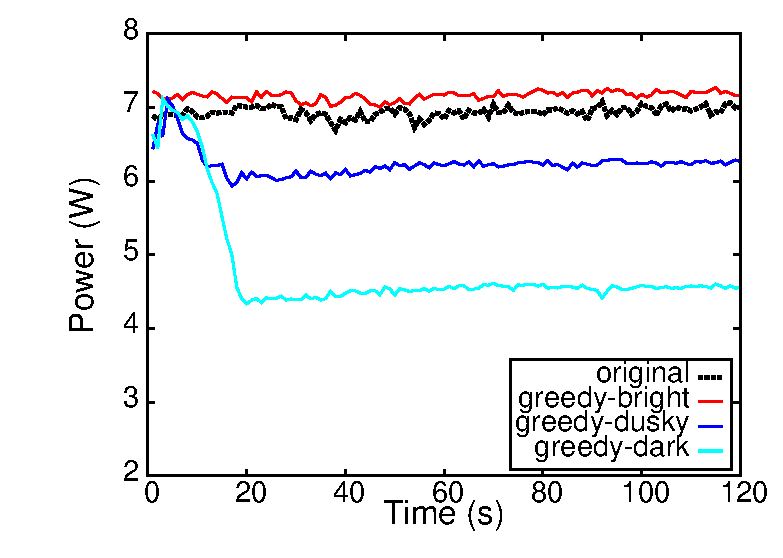
\includegraphics[scale=.6]{./figures/power.eps}
    \caption{Power consumption of the Samsung tablet during real-time video communication under different scenes.}
    \label{fig:power}
  \end{center}
  %\vspace{-3em}
\end{figure}


We measure the power consumption under scenes with different levels of
brightness.  These scenes are tagged with {\it bright}, {\it dusky}
and {\it dark}.  Under the {\it bright} scene, the maximum pixel
luminance of frames is close to 255, which leaves our LCD-GDP scheme
very little space for backlight scaling.  Under the {\it dusky} and
{\it dark} scenes, with smaller maximum luminance value (about 190 and
107, respectively), we can save more power by dimming the backlight
and maintain the observed brightness via luminance compensation.  We
compare the power consumption of our LCD-GDP scheme under different
scenes with the power consumption of the original version of WebRTC
app.  The results are shown in Figure~\ref{fig:power}.  Since the
power consumption of the original WebRTC app under different scenes is
almost the same, we only plot the result under bright environment in
this figure, which is $6.935$ watts on average.  This value is
considered as the baseline.  Under the same {\it bright} scene, and
the power consumption of our LCD-GDP is $7.160$ watts, slightly higher
than the baseline.  This is because extra modules are integrated into
the system, consuming more power, while the backlight is never dimmed
throughout the conversation.  In the {\it dusky} and {\it dark} scene
experiments, the backlight intensity is gradually dimmed by the greedy
algorithm, reducing the power consumption shown as the beginning
descendent gradient.  As a result, only $6.235$ watts and $4.783$
watts power is consumed on average, saving $12.92\%$ and $33.20\%$
power, respectively.
%

\subsection{Video Quality}

We next examine the quality of video calls made under our LCD-GDP
scheme. We focus four metrics frames per second (FPS), peak
signal to noise ratio (PSNR), structural similarity (SSIM), and user-perceived video call latency.
We compare our scheme with the original WebRTC app.

\noindent{\bf Frame Rate.} 
To measure the number of frames that are captured, encoded at the
sender side and decoded and rendered at the receiver side, we use the
statistics reported by the WebRTC app directly. We find that at the
sender side, the number of frames that are encoded varies
significantly if there are moving objects.  The frame rate reaches the
highest value when the frame content is a static scene.  Since our
scheme is agnostic to frame content, we only consider static scene in
our experiments.  This allows us to evaluate our scheme during video
call with a large number of frames per second.  We expect if our scheme
will not impact the video call with higher FPS, it will not impact the
calls with lower FPS either.  We set the resolution of captured video
to $640\times 480$ and measured the FPS under scenes with different
brightness.  Note that in the WebRTC app where we incorporated our
LCD-GDP scheme, the frame rate of generation is limited to $30$ FPS
and at most $15$ frames are rendered per second. In each experiment,
the video call lasted at least $5$ minutes. 
During the video call, the FPS metric is recorded every second. 
Then we report the statistical results of the FPS in different stages for the
video streaming originating from the Nexus smartphone to the Samsung tablet.



\begin{table}[t]
  \small
  \centering
  \caption{FPS of video stream originating from Nexus 4 smartphone to
    Samsung tablet.}
	\vspace{0.5em}
  \label{tab:fps}
  %% fps input | fps sent | fps received | fps decoded | fps output | sent bitrate | receive bitrate
  \begin{tabular}{|c||c|c||c|c||c|c|} %lcr
    \hline
%    & \multicolumn{6}{|c|}{FPS} \\ \hline
    & \multicolumn{2}{|c||}{Input} & \multicolumn{2}{|c||}{Sent}
    & \multicolumn{2}{|c|}{Output}
    \\ \hline
    & $E$ & $\delta$ & $E$ & $\delta$ & $E$ & $\delta$ \\ \hline
    \multicolumn{7}{|c|}{Bright scenario} \\ \hline
    Original App & $23.78$ & $1.66$ & $19.09$ & $2.81$ & $13.91$ & $4.41$ 
    \\ \hline
    LCD-GDP & $23.99$ & $1.18$ & $18.79$ & $3.06$ & $13.60$ & $3.17$
    \\ \hline
    \multicolumn{7}{|c|}{Dark scenario} \\ \hline
    Original App & $8.02$ & $1.37$ & $8.00$ & $0.42$ & $4.85$ & $0.72$ \\ \hline
    LCD-GDP & $7.85$ & $0.48$ & $8.00$ & $0.18$ & $4.96$ & $0.53$ \\ \hline
    %% & \multicolumn{2}{inputfps} & \multicolumn{2}{sentfps} & \multicolumn{2}{outputfps} & sentbitrate & recvbitrate \\ \hline
  \end{tabular}
  %\vspace{-18pt}  
\end{table}


Table~\ref{tab:fps} shows the frame rate of the video stream originated from the Nexus 4 smartphone 
in different stages. The {\it Input} column indicates the rate of frames captured at the camera. 
The {\it Sent} column indicates the frame rate of the encoded video stream.
This stream is sent over the network and decoded at the receiver side.
The final rendered frame rate is shown in the {\it Output} column. 
$E$ stands for the
expectation of the result and $\delta$ is the corresponding standard
deviation. The table shows that FPS is always lower in the dark scenario
even in the original scheme. We find this frame rate degradation
is due to the specific implementation of the original WebRTC app. Comparing these two
extreme cases in the lowest FPS and the highest FPS,  we find there is no degradation of video quality in terms of FPS.

\noindent{\bf Image Fidelity.} 	
Fidelity loss could occur in LCD-GDP for two reasons: (i) the maximum pixel luminance of 
frames increases abruptly, causing the constraint shown in Equation~\cite{eq:distort} be violated;
and (ii) the luminance information piggybacked in the delivered frames is lost due to video
compression or network transmission.
To measure video quality, we calculate the Peak
Signal-to-Noise Ratio (PSNR) and Structural SIMilarity (SSIM) 
between the receiver-observed video stream and the original stream captured at the sender. 
%At the sender side, we record the frames captured by the camera; 
%at the receiver side, we record the frames output from the rendering module.
To align the frames, we insert a black frame into the streaming every $10$ 
frames as the anchor. Then we record all the frames on both sides. 
We only compare the frames between two anchor frames if there 
are exactly $10$ frames recorded on both sides. 
The results are shown in the Table~\ref{tab:distortion}.

Using the original WebRTC app under Dusky Scene, for example, the PSNR and SSIM between 
the rendered frame and the original captured frame is 41.79 and 0.98, respectively. 
The difference is caused by video compression as expected. We use this value as baseline
and see if using the greedy algorithm causes more fidelity loss. 
The result show that the PSNR and SSIM of LCD-GDP under the same scene has the same
value of 41.79, indicating video quality is not affected.
Under the Bright Scene and the Dark Scene, the PSNR is slightly decreased using LCD-GDP.
However, the PSNR values are still above 40 dB, indicating there is very little distortion.

%Potentially, with LCD-GDP, there are two possible reasons that may
%cause the received frames to lose image fidelity: 1) the luminance
%information piggybacked in the delivered frames is lost due to video
%compression or network transmission, 2) the maximum luminance of
%consecutive frames increases abruptly. To investigate this potential
%quality loss, we measured the received video quality using both Peak
%Signal-to-Noise Ratio (PSNR) and Structure SIMilarity (SSIM). To align
%the frames, a black frame is inserted into the streaming every $10$
%frames as the anchor. Then we recorded all the frames on both
%sides. We only compare the frames between two anchor frames if there
%are exact $10$ frames recorded on both sides.  The resemblance of the
%frames is measured in the case of  original WebRTC implementation
%("Original" in the table), using dynamic programming for luminance
%adjustment ("DP" in the table), and our greedy algorithm ("Greedy" in
%the table).  We conducted this experiments under the same scenes where
%we performed the power consumption experiment. The length of the
%videos measured in  this experiment are all $3$ minutes. The results
%are shown in the Table~\ref{tab:distortion}.

%\begin{table}[t]
%  \small
%  \centering
%  \caption{Image fidelity}
%  
%  \begin{tabular}{|c|c|c|c|c|c|c|}
%    \hline
%    & \multicolumn{2}{|c|}{Original} & \multicolumn{2}{|c|}{DP} & \multicolumn{2}{|c|}{Greedy} \\ \hline
%    & $E$ & $\delta$ & $E$ & $\delta$ & $E$ & $\delta$ \\ \hline
%    \multicolumn{7}{|c|}{bright} \\ \hline
%    PSNR & 41.89 & 4.85 & 41.57 & 4.96 & 41.79 & 4.85 \\ \hline
%    SSIM & 0.98 & 0.01 & 0.98 & 0.01 & 0.98 & 0.01 \\ \hline
%    \multicolumn{7}{|c|}{dusky} \\ \hline
%    PSNR & 41.79 & 4.85 & 41.57 & 4.96 & 41.79 & 4.85 \\ \hline
%    SSIM & 0.98 & 0.01 & 0.98 & 0.01 & 0.98 & 0.01 \\ \hline
%    \multicolumn{7}{|c|}{dark} \\ \hline
%    PSNR & 44.86 & 6.88 & 41.63 & 9.62 & 41.63 & 9.78 \\ \hline
%    SSIM & 0.97 & 0.01 & 0.97 & 0.01 & 0.97 & 0.01 \\ \hline
%  \end{tabular}
%  \label{tab:distortion}
%\end{table}

%% In this table, we show the expectation and standard deviation in both
%% PSNR and SSIM respectively.  From the results of PSNR and SSIM, the
%% similarity of frames between sender and receiver stays almost same in
%% bright and dusky scenes. In the dark scenes, our scheme undermine the
%% resemblance of the images in PSNR. The reason is in the dark
%% environment, the frames transmitted have lower contrast. The luminance
%% information stored in the frames will lose in higher probability other
%% than the previous two cases. But the PSNR result of $41.63$ are still
%% a good rendered quality. So we can conclude that little distortion is
%% introduced into the video conferencing by applying our LCD-GDP.


\begin{table}[t]
	\small
	\centering
	\caption{PSNR (dB) and SSIM between the rendered video stream and the original captured frame.}
	\vspace{0.5em}
	\begin{tabular}{|c||c|c||c|c|}
		\hline
		& \multicolumn{2}{|c||}{Original WebRTC App} & \multicolumn{2}{|c|}{LCD-GDP} \\ \hline
		& $E$ & $\delta$ & $E$ & $\delta$ \\ \hline
		\multicolumn{5}{|c|}{Bright Scene} \\ \hline
		PSNR & 41.89 & 4.85 & 41.79 & 4.85 \\ \hline
		SSIM & 0.98 & 0.01  & 0.98 & 0.01 \\ \hline
		\multicolumn{5}{|c|}{Dusky Scene} \\ \hline
		PSNR & 41.79 & 4.85  & 41.79 & 4.85 \\ \hline
		SSIM & 0.98 & 0.01  & 0.98 & 0.01 \\ \hline
		\multicolumn{5}{|c|}{Dark Scene} \\ \hline
		PSNR & 44.86 & 6.88  & 41.63 & 9.78 \\ \hline
		SSIM & 0.97 & 0.01  & 0.97 & 0.01 \\ \hline
	\end{tabular}
	\label{tab:distortion}
        %\vspace{-18pt}  
\end{table}


%From the table, we can see in the dusky setting, the PSNR for
%original, DP, and Greedy is $41.89\pm4.85$, $41.57\pm4.96$ and
%$41.79\pm4.85$ respectively. The DP and the Greedy algorithm both make
%no promotion on this metric. The corresponding SSIM values are all
%$0.98\pm0.01$, confirming that there is no difference perceived by the
%user. Similar results are observed in the case of bright and dark
%cases.


\noindent{\bf User-perceived Video Latency.} 
We also measure the user-perceived video call delay.
To minimize the impact of wide area network dynamics, 
we conduct the experiments in the same local area network (LAN).
%At last, the communication latency is also measured between these two machines. 
To measure the end-to-end delay, 
we place the camera on the mobile device in front of a stop watch
and compare the timestamps rendered on two devices using the method proposed by Yu et al.~\cite{6848080}. 
In the original WebRTC app, we find the average latency is $261$ milliseconds 
during the video call. When the LCD-GDP scheme is applied, the average latency
is increased to $302$ milliseconds, indicating only about $40$ milliseconds delay are
introduced due to the additional processing. 


%% \begin{table}[h]
%%   \centering
%%   \caption{video latency}
%%   \label{tab:latency}
%%   \begin{tabular}{|c|c|}
%%     \hline
%%     & latency (ms) \\ \hline
%%     Original & 261 \\ \hline
%%     Greedy & 302 \\ \hline
%%   \end{tabular}
%% \end{table}



%% The Table~\ref{tab:latency} shows the latency measured under different
%% schemes in milliseconds. From the result, the scanning operation and
%% the greedy determination stage introduce minor latency, about tens of
%% milliseconds into video conferencing. 




%% We conducted all the experiments on two devices: one NEXUS 4
%% smartphone and one Samsung Galaxy 10.1-inch tablet. We first examine
%% how much energy can we saved by using the LCD-GDP during the real-time
%% communication. As the
%% additional stages are added into the video conferencing, we then
%% evaluate if our implementation will impact the video streaming
%% quality. Finally we measured if our scheme will introduce distortion
%% into the video calls. 

%% \subsection{Power Consumption}

%% \begin{figure}[t]
%%   \begin{center}
%%   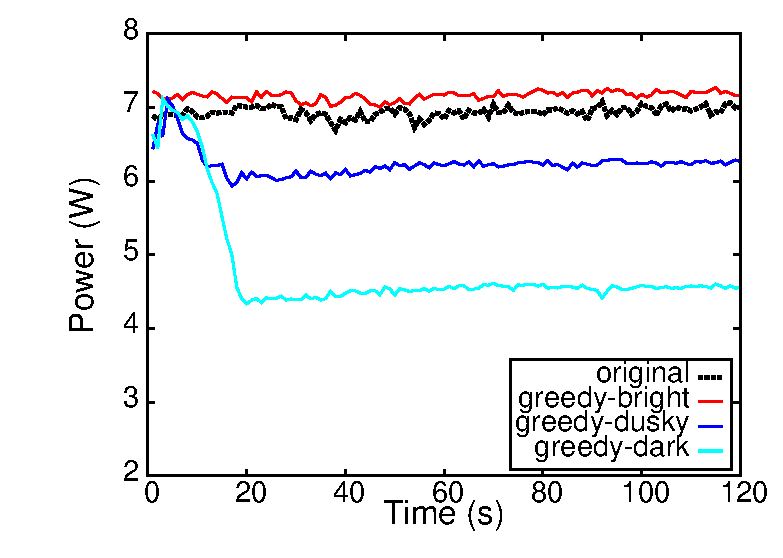
\includegraphics[scale=.5]{./figures/power.eps}
%%   \caption{Power consumption of real-time communication}
%%   \label{fig:power}
%%   \end{center}
%% \end{figure}


%% We measured the power consumption of the real-time
%% communication between these two devices. To evaluate the
%% effect of our system, we test the power consumption under scenes with
%% different levels of brightness. A two-minute conversation is conducted
%% in each experiment. The scenes can be tagged with {\it bright}, {\it
%%   dusky} and {\it dark}, which make backlight level set to $0.99$,
%% $0.75$ and $0.42$ on average in our system. Also we measured the power
%% consumption of the original version of WebRTC app. The results are
%% plot on figure~\ref{fig:power}. The x-axis is the time in seconds, and
%% the y-axis is the power consumption in walts. In this figure, power
%% consumption of the original WebRTC app under different scenes is
%% almost in same level so only the result under bright environment is
%% plot, which is $6.935$ walts on average. This value is considered as
%% the baseline and the power consumption of our system is found slightly
%% higher than it, which is $7.160$ walts. The reason is that extra
%% modules are integrated into the system but the backlight has never
%% been dimmed across the conversation. In the dusky and dark case,
%% $6.235$ ($12.92\%$) walts and $4.783$ ($33.20\%$) walts is consumed on
%% average by dimming the backlight intensity. The beginning descendent
%% gradient shows the process of the greedy algorithm dimming the
%% backlight intensity.


%% \subsection{Video quality}
%% In worrying about our scheme will make the quality of the video calls
%% degrade, we measured the quality metrics in frames per second (fps)
%% and latency. The comparison is made by our greedy scheme and the
%% original version. All the results are reported by the webRTC app
%% itself. 

%% In the measurement, the fps metric varied in great range if moving
%% objects is involved into the frames. The frame rate reached the
%% highest threshold if the frame content is a static scene. Only the
%% static scene is used in our experiment.  We expect if our scheme will
%% not impact the video streaming with higher fps, it won't impact the
%% one with lower fps as well. We measured the fps under scenes with
%% different brightness and the resolution of the video streaming is set as
%% $640$x$480$. In the webRTC app, the frame rate of generation is
%% limited to $30$ fps and at most $15$ frames are rendered per
%% second. At least $5$ minutes streaming is maintained in each
%% experiment. The data is collected from the Samsung tablet. 


%% \begin{table}[h]
%%   \centering
%%   \caption{video frames per second}
%%   \label{tab:fps}
%%   %% fps input | fps sent | fps received | fps decoded | fps output | sent bitrate | receive bitrate
%%   \begin{tabular}{|c|c|c|c|c|c|c|} %lcr
%%     \hline
%%     & \multicolumn{6}{|c|}{fps} \\ \hline
%%     & \multicolumn{2}{|c|}{input} & \multicolumn{2}{|c|}{sent}
%%     & \multicolumn{2}{|c|}{output}
%%     \\ \hline
%%     & $E$ & $\delta$ & $E$ & $\delta$ & $E$ & $\delta$ \\ \hline
%%     \multicolumn{7}{|c|}{bright scenario} \\ \hline
%%     original & $23.78$ & $1.66$ & $19.09$ & $2.81$ & $13.91$ & $4.41$ 
%%     \\ \hline
%%     greedy & $23.99$ & $1.18$ & $18.79$ & $3.06$ & $13.60$ & $3.17$
%%     \\ \hline
%%     \multicolumn{7}{|c|}{dark scenario} \\ \hline
%%     original & $8.02$ & $1.37$ & $8.00$ & $0.42$ & $4.85$ & $0.72$ \\ \hline
%%     greedy & $7.85$ & $0.48$ & $8.00$ & $0.18$ & $4.96$ & $0.53$ \\ \hline
%%     %% & \multicolumn{2}{inputfps} & \multicolumn{2}{sentfps} & \multicolumn{2}{outputfps} & sentbitrate & recvbitrate \\ \hline
%%   \end{tabular}
  
%% \end{table}


%% In the Table~\ref{tab:fps}, we show the fps of the video in different
%% stages. The {\it input} tag means the frame generation rate of the
%% capturer. {\it sent} and {\it output} means the network sent rate and
%% final rendering frame rate respectively. $E$ stands for the
%% expectation of the result and $\delta$ is the corresponding standard
%% deviation. From this table, fps is always lower in the dark scenario
%% even in the original scheme. We can conclude this quality degradation
%% is due to the specific implementation of this app. Comparing these two
%% extreme cases in the lowest fps and the highest fps, there is no
%% degradation of the video quality in fps is found. 

%% The communication latency is also measured between these two
%% machine. We use the method proposed in~\cite{yu2014can}. In the
%% original version, $261$ milliseconds of latency on average is found
%% during the video call. When applying the LCD-GDP, the average latency
%% increases to $302$ milliseconds. Only $40$ milliseconds are
%% introduced. 


%% To evaluate the power consumption of our system, we setup the devices
%% under scenes with different brightness and the power consumption of
%% the tablet is measured by the power monitor. The results are shown in
%% ~\ref{tab:power_consumption}.
 
%% installed the original version WebRTC app and an upgraded version
%% equipped with our dynamic programming scheme. When these two devices
%% connected to each other, we put them under different environments to
%% evaluate if our scheme could outperform the original version. Two
%% extreme environments were selected purposely. One was an extreme
%% bright environment that our scheme didn't work any more. Under the
%% other environment, which is an extreme dark case, the backlight could
%% always be scaled to the lowest threshold($0.4$).
%% We measured the power
%% consumption of the tablets in all of these cases and the results are
%% shown in ~\ref{tab:power_consumption}.


%% \begin{table}[h]
%%   \centering
%%   \caption{power consumption}
%%   \label{tab:power_consumption}
%%   %% device | dark | bright |
%%   \begin{tabular}{|c|c|c|c|c|} %lcr
%%     \hline
%%     & \multicolumn{2}{|c|}{SAMSUNG(dark)} & \multicolumn{2}{|c|}{SAMSUNG(bright)} \\ \hline
%%     & no-adaption & with adaption & no-adaption & with adaption \\ \hline
%%     NEXUS(dark) & $\sim{6250}$ mW & $\sim{3810}$ mW & $\sim{6900}$ mW & $\sim{4150}$ mW  \\ \hline
%%     NEXUS(bright) & $\sim{6500}$ mW & $\sim{6400}$ mW & $\sim{7250}$ mW & $\sim{6800}$ mW \\ \hline
%%   \end{tabular}
  
%% \end{table}

%% From the table, we found that the original version WebRTC app consumed
%% similar power, which was from $6250$ mA to $7250$ mA, under different
%% environments. The slight difference are caused by the mutable fps. The
%% WebRTC app actively reduces the fps if it detects that the environment
%% gets dark. So the power consumption was found lowest when both the
%% devices were put in the dark environment. The most observable power
%% savings were found in the case that the NEXUS was put in the dark
%% environment. The dimmed frames sent by the NEXUS help the tablet take
%% advantage of the luminance compensation technique.  Notice that
%% although our scheme outperformed the original version in the both
%% bright case. This power reduction comes from the lower fps. The
%% dynamic programming algorithm, holding too many frames before
%% delivering them to the rendering module, will definitely degrade the
%% video quality.

%% \begin{table}[h]
%%   \centering
%%   \caption{power consumption}
%%   \label{tab:power_consumption}
%%   %% device | dark | bright |
%%   \begin{tabular}{|c|c|c|c|c|} %lcr
%%     \hline
%%     & \multicolumn{2}{|c|}{SAMSUNG(dark)} & \multicolumn{2}{|c|}{SAMSUNG(bright)} \\ \hline
%%     & no-adaption & with adaption & no-adaption & with adaption \\ \hline
%%     NEXUS(dark) & $\sim{6250}$ mW & $\sim{3810}$ mW & $\sim{6900}$ mW & $\sim{4150}$ mW  \\ \hline
%%     NEXUS(bright) & $\sim{6500}$ mW & $\sim{6400}$ mW & $\sim{7250}$ mW & $\sim{6800}$ mW \\ \hline
%%   \end{tabular}
  
%% \end{table}


%% Expr 1:
%% Comparison between normal case and cases applied our scheme.
%% Prove that our implementation doesn't downgrade the user experience.
%% \begin{itemize}
%%   \item{bitrate}
%%   \item{fps}
%%   \item{maybe others}
%% \end{itemize}

%% Expr 2:
%% Compare the distortion of frames among 1) normal case 2) DP 3)
%% Greedy. store the frames under different brightness. (90\%-100\%,
%% 70\%-80\%, 50\%-60\%).
%% To align the frames. (Can try index the frames in several pixels)
%% \begin{itemize}
%%   \item{PSNR}
%%   \item{SSIM}
%% \end{itemize}



%% The
%% dynamic programming algorithm has to hold enough frames to adjust
%% backlight, so that it can not deliver the frames to the rendering
%% module in time.


%% quality of the video in webRTC is self-adjusted. There are two factors
%% affecting the fps and bitrate: the average luminance of the frames and
%% the content of the frames. The webRTC app intends to reduce the
%% fps/bitrate in darker images. Also the static frames gains higher
%% fps/bitrate other than the frames containing moving objects. To
%% evaluate how much overhead is introduced by our scheme, we only use
%% the static scenario as the test case. We expect if our greedy
%% algorithm won't impair the visual quality of the static scenario,
%% which features higher fps and bitrate, the quality of scenarios
%% containing moving objects will not be damaged as well.



%% \begin{table}[h]
%%   \centering
%%   \caption{video quality}
%%   \label{tab:quality}
%%   %% fps input | fps sent | fps received | fps decoded | fps output | sent bitrate | receive bitrate
%%   \begin{tabular}{|c|c|c|c|c|c|c|c|c|} %lcr
%%     \hline
%%     & \multicolumn{6}{|c|}{fps} & \multicolumn{2}{|c|}{bitrate} \\ \hline
%%     & \multicolumn{2}{|c|}{input} & \multicolumn{2}{|c|}{sent}
%%     & \multicolumn{2}{|c|}{output} & sent & recv
%%     \\ \hline
%%     & $E$ & $\delta$ & $E$ & $\delta$ & $E$ & $\delta$ & & \\ \hline
%%     \multicolumn{9}{|c|}{bright scenario/loopback} \\ \hline
%%     original & $24.67$ & $1.01$ & $22.73$ & $3.59$ & $15.37$ & $2.44$ &
%%     $81076$ & $81344$ \\ \hline
%%     greedy & $24.51$ & $1.06$ & $21.64$ & $2.76$ & $15.19$ & $2.06$ &
%%     $44832$ & $45193$ \\ \hline
%%     \multicolumn{9}{|c|}{bright scenario/remote} \\ \hline
%%     original & $23.78$ & $1.66$ & $19.09$ & $2.81$ & $13.91$ & $4.41$ &
%%     $269094$ & $41583$ \\ \hline
%%     greedy & $23.99$ & $1.18$ & $18.79$ & $3.06$ & $13.60$ & $3.17$ &
%%     $267309$ & $32905$ \\ \hline
%%     \multicolumn{9}{|c|}{dark scenario/loopback} \\ \hline
%%     original & $7.86$ & $0.35$ & $8.00$ & $0.00$ & $7.87$ & $0.40$ &
%%     $168306$ & $168306$ \\ \hline
%%     greedy & $7.88$ & $0.39$ & $8.00$ & $0.05$ & $7.87$ & $0.39$ &
%%     $165936$ & $165936$ \\ \hline
%%     \multicolumn{9}{|c|}{dark scenario/remote} \\ \hline
%%     original & $8.02$ & $1.37$ & $8.00$ & $0.42$ & $4.85$ & $0.72$ &
%%     $462505$ & $924722$ \\ \hline
%%     greedy & $7.85$ & $0.48$ & $8.00$ & $0.18$ & $4.96$ & $0.53$ &
%%     $246837$ & $779452$ \\ \hline
%%     %% & \multicolumn{2}{inputfps} & \multicolumn{2}{sentfps} & \multicolumn{2}{outputfps} & sentbitrate & recvbitrate \\ \hline
%%   \end{tabular}
  
%% \end{table}

%% Two devices are used in this measurement, one Samsung 10.1-inch tablet
%% and one NEXUS 4 smartphone. The data is collected from the tablet. We test the
%% real-time communication in the resolution of $640$x$480$, and set the
%% upperbound of the frames generation by the camera as $30$. Both the
%% dark scenario and the bright scenario are measured. We maintained the
%% communication at least $5$ minutes. We test the {\it loopback} and the
%% {\it remote} respectively. The {\it loopback} means the tablet
%% communicate to itself via network. And the {\it remote} means
%% communication between two devices.


\section{conclusion}
\label{sec:conclusion}

In this paper, we explored the possibility of applying backlight
scaling technique for real-time communication on the mobile devices,
and proposed the LCD-GDP to reduce the power consumption during the
video calls. We identified the challenges of efficiently migrating the
computation intensive tasks from offline to online. In order to scan
each frame for generating luminance histogram only once, we located
the scanning module at sender side and piggybacked this luminance
information in duplicated way. We also used a greedy algorithm to
replace the commonly applied dynamic programming technique. This would
not introduce significant latency into the communication. Finally, we
take advantage of the GPU to compensate the pixel luminance in an
timely manner. We built our LCD-GDP based on the WebRTC implementation
of chrome and evaluate it as an Anroid app. From the evaluation, upto
$33\%$ power consumption is saved on average by using our LCD-GDP. At
the same time, the quality of services in fps and latency stay in the
same level as the original real-time streaming. Little distortion in
PSNR and SSIM is found in the LCD-GDP.



%------------------------------------------------------------------------------

\bibliographystyle{IEEEtran}

{
% \begin{footnotesize}
   \bibliography{display}
% \end{footnotesize}
}

%------------------------------------------------------------------------------

%\input{appendix}


%------------------------------------------------------------------------------

\end{document}

%------------------------------------------------------------------------------ 
